\documentclass[border=8pt]{standalone}
\usepackage[T1]{fontenc}\usepackage{helvet}\renewcommand{\familydefault}{\sfdefault}
\usepackage{tikz}\usetikzlibrary{arrows.meta, positioning, calc, backgrounds}
\definecolor{ink}{HTML}{1a1916}
\definecolor{inktwo}{HTML}{3a3a35}
\definecolor{inkthree}{HTML}{6a6862}
\definecolor{rule}{HTML}{b8b09a}
\definecolor{amber}{HTML}{a8730a}
\definecolor{red}{HTML}{c8261a}
\definecolor{paper}{HTML}{f0eee5}
\definecolor{slab}{HTML}{d8d4c6}
\tikzset{
  >={Stealth[length=2.2mm]},
  wire/.style={line width=0.8pt, ink},
  modwire/.style={line width=0.6pt, dashed, ink},
  tastewire/.style={line width=0.6pt, dashed, amber},
  gatewire/.style={line width=0.6pt, dotted, ink},
  block/.style={rectangle, draw=ink, line width=0.9pt, fill=slab, minimum width=3.0cm, minimum height=1.9cm, inner sep=0pt},
  perf/.style={rectangle, draw=ink, line width=0.7pt, minimum width=3.0cm, minimum height=0.7cm, inner sep=2pt, font=\footnotesize, text=ink},
  title/.style={font=\scriptsize\bfseries, text=ink, anchor=north, inner sep=2pt},
  jack/.style={circle, draw=ink, fill=paper, line width=0.5pt, minimum size=3.2pt, inner sep=0pt},
  plabel/.style={font=\tiny, text=inktwo, anchor=west, inner sep=1pt},
  olabel/.style={font=\tiny, text=inktwo, anchor=east, inner sep=1pt},
  settings/.style={font=\scriptsize, text=ink, align=left, anchor=north west, inner sep=1pt, text width=2.9cm},
}
\begin{document}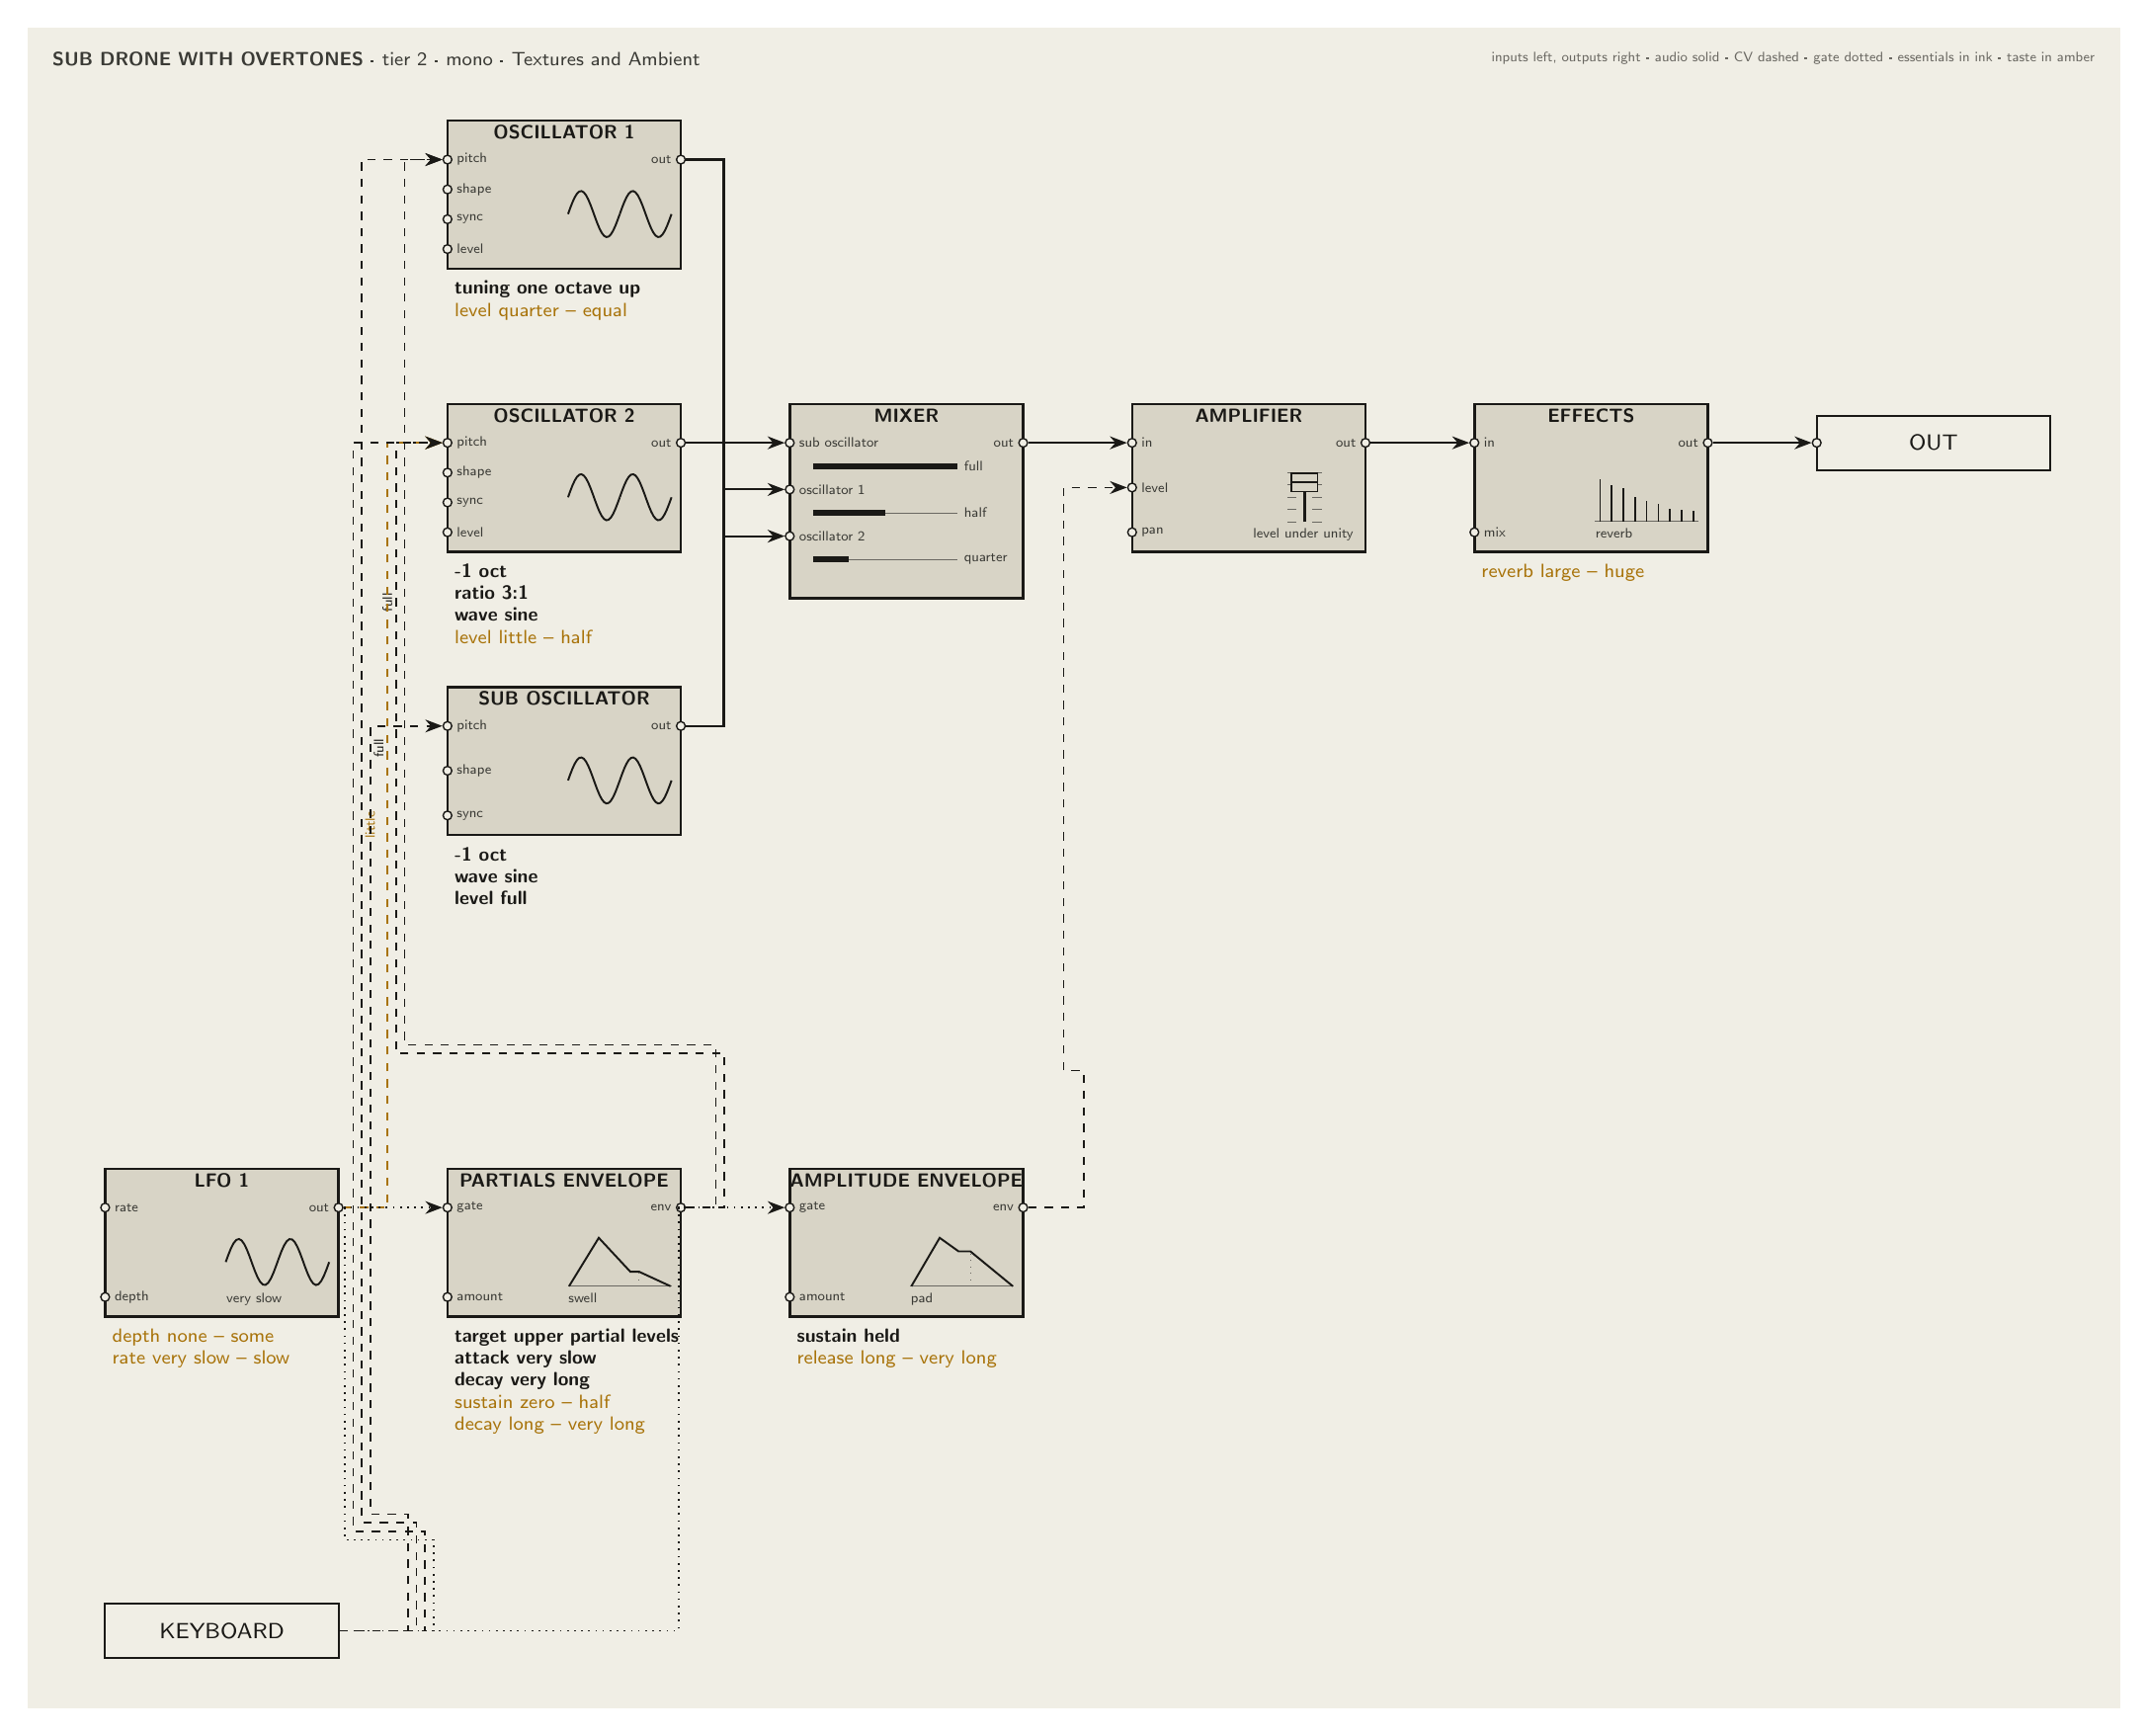
\begin{tikzpicture}
\begin{scope}[on background layer]\fill[paper] (-2.5,-15.819999999999999) rectangle (24.4,5.79);\end{scope}
\node[block, minimum height=1.9cm] (osc1) at (4.4,3.6399999999999997) {};
\node[title] at (osc1.north) {OSCILLATOR 1};
\node[jack] (osc1-pitch) at (2.9000000000000004,4.09) {};
\node[plabel] at (2.9800000000000004,4.09) {pitch};
\node[jack] (osc1-shape) at (2.9000000000000004,3.7066666666666666) {};
\node[plabel] at (2.9800000000000004,3.7066666666666666) {shape};
\node[jack] (osc1-sync) at (2.9000000000000004,3.3233333333333333) {};
\node[plabel] at (2.9800000000000004,3.3233333333333333) {sync};
\node[jack] (osc1-level) at (2.9000000000000004,2.94) {};
\node[plabel] at (2.9800000000000004,2.94) {level};
\node[jack] (osc1-out) at (5.9,4.09) {};
\node[olabel] at (5.82,4.09) {out};
\begin{scope}
\draw[ink, line width=0.7pt] plot[domain=0.000:0.500, samples=24, variable=\u] ({4.450+\u*1.330},{3.020+(0.740)*(0.5+0.4*sin(360*(\u*2))+0.0)});
\draw[ink, line width=0.7pt] plot[domain=0.500:1.000, samples=24, variable=\u] ({4.450+\u*1.330},{3.020+(0.740)*(0.5+0.4*sin(360*(\u*2))+0.0)});
\end{scope}
\node[settings] at (2.95,2.5699999999999994) {\textbf{tuning one octave up} \\ \textcolor{amber}{level quarter -- equal}};
\node[block, minimum height=1.9cm] (osc2) at (4.4,0.0) {};
\node[title] at (osc2.north) {OSCILLATOR 2};
\node[jack] (osc2-pitch) at (2.9000000000000004,0.44999999999999996) {};
\node[plabel] at (2.9800000000000004,0.44999999999999996) {pitch};
\node[jack] (osc2-shape) at (2.9000000000000004,0.06666666666666665) {};
\node[plabel] at (2.9800000000000004,0.06666666666666665) {shape};
\node[jack] (osc2-sync) at (2.9000000000000004,-0.31666666666666665) {};
\node[plabel] at (2.9800000000000004,-0.31666666666666665) {sync};
\node[jack] (osc2-level) at (2.9000000000000004,-0.7) {};
\node[plabel] at (2.9800000000000004,-0.7) {level};
\node[jack] (osc2-out) at (5.9,0.44999999999999996) {};
\node[olabel] at (5.82,0.44999999999999996) {out};
\begin{scope}
\draw[ink, line width=0.7pt] plot[domain=0.000:0.500, samples=24, variable=\u] ({4.450+\u*1.330},{-0.620+(0.740)*(0.5+0.4*sin(360*(\u*2))+0.0)});
\draw[ink, line width=0.7pt] plot[domain=0.500:1.000, samples=24, variable=\u] ({4.450+\u*1.330},{-0.620+(0.740)*(0.5+0.4*sin(360*(\u*2))+0.0)});
\end{scope}
\node[settings] at (2.95,-1.0699999999999998) {\textbf{-1 oct} \\ \textbf{ratio 3:1} \\ \textbf{wave sine} \\ \textcolor{amber}{level little -- half}};
\node[block, minimum height=1.9cm] (sub) at (4.4,-3.6399999999999997) {};
\node[title] at (sub.north) {SUB OSCILLATOR};
\node[jack] (sub-pitch) at (2.9000000000000004,-3.1899999999999995) {};
\node[plabel] at (2.9800000000000004,-3.1899999999999995) {pitch};
\node[jack] (sub-shape) at (2.9000000000000004,-3.7649999999999997) {};
\node[plabel] at (2.9800000000000004,-3.7649999999999997) {shape};
\node[jack] (sub-sync) at (2.9000000000000004,-4.34) {};
\node[plabel] at (2.9800000000000004,-4.34) {sync};
\node[jack] (sub-out) at (5.9,-3.1899999999999995) {};
\node[olabel] at (5.82,-3.1899999999999995) {out};
\begin{scope}
\draw[ink, line width=0.7pt] plot[domain=0.000:0.500, samples=24, variable=\u] ({4.450+\u*1.330},{-4.260+(0.740)*(0.5+0.4*sin(360*(\u*2))+0.0)});
\draw[ink, line width=0.7pt] plot[domain=0.500:1.000, samples=24, variable=\u] ({4.450+\u*1.330},{-4.260+(0.740)*(0.5+0.4*sin(360*(\u*2))+0.0)});
\end{scope}
\node[settings] at (2.95,-4.71) {\textbf{-1 oct} \\ \textbf{wave sine} \\ \textbf{level full}};
\node[block, minimum height=2.5cm] (mix) at (8.8,-0.30000000000000004) {};
\node[title] at (mix.north) {MIXER};
\node[jack] (mix-sub) at (7.300000000000001,0.44999999999999996) {};
\node[plabel] at (7.380000000000001,0.44999999999999996) {sub oscillator};
\draw[inkthree, line width=0.3pt] (7.600,0.150) -- (9.450,0.150);
\draw[ink, line width=2.2pt] (7.600,0.150) -- (9.450,0.150);
\node[font=\tiny, text=inktwo, anchor=west, inner sep=1pt] at (9.500,0.150) {full};
\node[jack] (mix-osc1) at (7.300000000000001,-0.15000000000000002) {};
\node[plabel] at (7.380000000000001,-0.15000000000000002) {oscillator 1};
\draw[inkthree, line width=0.3pt] (7.600,-0.450) -- (9.450,-0.450);
\draw[ink, line width=2.2pt] (7.600,-0.450) -- (8.525,-0.450);
\node[font=\tiny, text=inktwo, anchor=west, inner sep=1pt] at (9.500,-0.450) {half};
\node[jack] (mix-osc2) at (7.300000000000001,-0.75) {};
\node[plabel] at (7.380000000000001,-0.75) {oscillator 2};
\draw[inkthree, line width=0.3pt] (7.600,-1.050) -- (9.450,-1.050);
\draw[ink, line width=2.2pt] (7.600,-1.050) -- (8.062,-1.050);
\node[font=\tiny, text=inktwo, anchor=west, inner sep=1pt] at (9.500,-1.050) {quarter};
\node[jack] (mix-out) at (10.3,0.44999999999999996) {};
\node[olabel] at (10.22,0.44999999999999996) {out};
\node[block, minimum height=1.9cm] (amp) at (13.200000000000001,0.0) {};
\node[title] at (amp.north) {AMPLIFIER};
\node[jack] (amp-in) at (11.700000000000001,0.44999999999999996) {};
\node[plabel] at (11.780000000000001,0.44999999999999996) {in};
\node[jack] (amp-level) at (11.700000000000001,-0.125) {};
\node[plabel] at (11.780000000000001,-0.125) {level};
\node[jack] (amp-pan) at (11.700000000000001,-0.7) {};
\node[plabel] at (11.780000000000001,-0.7) {pan};
\node[jack] (amp-out) at (14.700000000000001,0.44999999999999996) {};
\node[olabel] at (14.620000000000001,0.44999999999999996) {out};
\begin{scope}
\draw[ink, line width=1.2pt] (13.915,-0.570) -- (13.915,0.070);
\draw[inkthree, line width=0.3pt] (13.695,-0.570) -- (13.815,-0.570) (14.015,-0.570) -- (14.135,-0.570);
\draw[inkthree, line width=0.3pt] (13.695,-0.410) -- (13.815,-0.410) (14.015,-0.410) -- (14.135,-0.410);
\draw[inkthree, line width=0.3pt] (13.695,-0.250) -- (13.815,-0.250) (14.015,-0.250) -- (14.135,-0.250);
\draw[inkthree, line width=0.3pt] (13.695,-0.090) -- (13.815,-0.090) (14.015,-0.090) -- (14.135,-0.090);
\draw[inkthree, line width=0.3pt] (13.695,0.070) -- (13.815,0.070) (14.015,0.070) -- (14.135,0.070);
\fill[slab, draw=ink, line width=0.6pt] (13.745,-0.178) rectangle (14.085,0.062);
\draw[ink, line width=0.5pt] (13.745,-0.058) -- (14.085,-0.058);
\node[font=\tiny, text=inktwo, anchor=north west, inner sep=0pt] at (13.250,-0.650) {level under unity};
\end{scope}
\node[block, minimum height=1.9cm] (fx) at (17.6,0.0) {};
\node[title] at (fx.north) {EFFECTS};
\node[jack] (fx-in) at (16.1,0.44999999999999996) {};
\node[plabel] at (16.18,0.44999999999999996) {in};
\node[jack] (fx-mix) at (16.1,-0.7) {};
\node[plabel] at (16.18,-0.7) {mix};
\node[jack] (fx-out) at (19.1,0.44999999999999996) {};
\node[olabel] at (19.020000000000003,0.44999999999999996) {out};
\begin{scope}
\draw[inkthree, line width=0.3pt] (17.650,-0.561) -- (18.980,-0.561);
\draw[ink, line width=0.6pt] (17.717,-0.561) -- (17.717,-0.018);
\draw[ink, line width=0.6pt] (17.866,-0.561) -- (17.866,-0.095);
\draw[ink, line width=0.6pt] (18.016,-0.561) -- (18.016,-0.133);
\draw[ink, line width=0.6pt] (18.165,-0.561) -- (18.165,-0.246);
\draw[ink, line width=0.6pt] (18.315,-0.561) -- (18.315,-0.296);
\draw[ink, line width=0.6pt] (18.465,-0.561) -- (18.465,-0.335);
\draw[ink, line width=0.6pt] (18.614,-0.561) -- (18.614,-0.394);
\draw[ink, line width=0.6pt] (18.764,-0.561) -- (18.764,-0.408);
\draw[ink, line width=0.6pt] (18.913,-0.561) -- (18.913,-0.429);
\node[font=\tiny, text=inktwo, anchor=north west, inner sep=0pt] at (17.650,-0.650) {reverb};
\end{scope}
\node[settings] at (16.150000000000002,-1.0699999999999998) {\textcolor{amber}{reverb large -- huge}};
\node[block, minimum height=1.9cm] (lfo1) at (0.0,-9.83) {};
\node[title] at (lfo1.north) {LFO 1};
\node[jack] (lfo1-rate) at (-1.5,-9.38) {};
\node[plabel] at (-1.42,-9.38) {rate};
\node[jack] (lfo1-depth) at (-1.5,-10.530000000000001) {};
\node[plabel] at (-1.42,-10.530000000000001) {depth};
\node[jack] (lfo1-out) at (1.5,-9.38) {};
\node[olabel] at (1.42,-9.38) {out};
\begin{scope}
\draw[ink, line width=0.7pt] plot[domain=0:1, samples=40, variable=\u] ({0.050+\u*1.330},{-10.450+(0.740)*(0.5+0.4*sin(360*\u*2))});
\node[font=\tiny, text=inktwo, anchor=north west, inner sep=0pt] at (0.050,-10.480) {very slow};
\end{scope}
\node[settings] at (-1.45,-10.899999999999999) {\textcolor{amber}{depth none -- some} \\ \textcolor{amber}{rate very slow -- slow}};
\node[block, minimum height=1.9cm] (menv) at (4.4,-9.83) {};
\node[title] at (menv.north) {PARTIALS ENVELOPE};
\node[jack] (menv-gate) at (2.9000000000000004,-9.38) {};
\node[plabel] at (2.9800000000000004,-9.38) {gate};
\node[jack] (menv-amount) at (2.9000000000000004,-10.530000000000001) {};
\node[plabel] at (2.9800000000000004,-10.530000000000001) {amount};
\node[jack] (menv-out) at (5.9,-9.38) {};
\node[olabel] at (5.82,-9.38) {env};
\begin{scope}
\draw[inkthree, line width=0.3pt] (4.450,-10.391) -- (5.780,-10.391);
\draw[ink, line width=0.7pt] (4.463,-10.391) -- (4.845,-9.769) -- (5.250,-10.204) -- (5.362,-10.204) -- (5.767,-10.391);
\draw[inkthree, line width=0.3pt, dotted] (5.362,-10.391) -- (5.362,-10.204);
\node[font=\tiny, text=inktwo, anchor=north west, inner sep=0pt] at (4.450,-10.480) {swell};
\end{scope}
\node[settings] at (2.95,-10.899999999999999) {\textbf{target upper partial levels} \\ \textbf{attack very slow} \\ \textbf{decay very long} \\ \textcolor{amber}{sustain zero -- half} \\ \textcolor{amber}{decay long -- very long}};
\node[block, minimum height=1.9cm] (aenv) at (8.8,-9.83) {};
\node[title] at (aenv.north) {AMPLITUDE ENVELOPE};
\node[jack] (aenv-gate) at (7.300000000000001,-9.38) {};
\node[plabel] at (7.380000000000001,-9.38) {gate};
\node[jack] (aenv-amount) at (7.300000000000001,-10.530000000000001) {};
\node[plabel] at (7.380000000000001,-10.530000000000001) {amount};
\node[jack] (aenv-out) at (10.3,-9.38) {};
\node[olabel] at (10.22,-9.38) {env};
\begin{scope}
\draw[inkthree, line width=0.3pt] (8.850,-10.391) -- (10.180,-10.391);
\draw[ink, line width=0.7pt] (8.863,-10.391) -- (9.227,-9.769) -- (9.470,-9.943) -- (9.621,-9.943) -- (10.167,-10.391);
\draw[inkthree, line width=0.3pt, dotted] (9.621,-10.391) -- (9.621,-9.943);
\node[font=\tiny, text=inktwo, anchor=north west, inner sep=0pt] at (8.850,-10.480) {pad};
\end{scope}
\node[settings] at (7.3500000000000005,-10.899999999999999) {\textbf{sustain held} \\ \textcolor{amber}{release long -- very long}};
\node[perf] (key) at (0.0,-14.819999999999999) {KEYBOARD};
\node[perf, fill=paper] (out) at (22.0,0.44999999999999996) {OUT}; \node[jack] (out-in) at (20.5,0.44999999999999996) {};
\draw[wire,->] (sub-out) -- (6.45,-3.1899999999999995) |- (mix-sub);
\draw[wire,->] (osc1-out) -- (6.45,4.09) |- (mix-osc1);
\draw[wire,->] (osc2-out) -- (6.45,0.44999999999999996) |- (mix-osc2);
\draw[wire,->] (mix-out) -- (10.850000000000001,0.44999999999999996) |- (amp-in);
\draw[wire,->] (amp-out) -- (fx-in);
\draw[wire,->] (fx-out) -- (out-in);
\draw[modwire,->] (menv-out) -- (6.3500000000000005,-9.38) -- (6.3500000000000005,-7.290000000000001) -- (2.3500000000000005,-7.290000000000001) -- (2.3500000000000005,4.09) -- (osc1-pitch);
\node[font=\tiny, text=ink, anchor=south, inner sep=1pt, rotate=90] at (2.2300000000000004,-1.6000000000000005) {full};
\draw[modwire,->] (menv-out) -- (6.460000000000001,-9.38) -- (6.460000000000001,-7.400000000000001) -- (2.2400000000000007,-7.400000000000001) -- (2.2400000000000007,0.44999999999999996) -- (osc2-pitch);
\node[font=\tiny, text=ink, anchor=south, inner sep=1pt, rotate=90] at (2.1200000000000006,-3.4750000000000005) {full};
\draw[tastewire,->] (lfo1-out) -- (2.1300000000000003,-9.38) -- (2.1300000000000003,0.44999999999999996) -- (osc2-pitch);
\node[font=\tiny, text=amber, anchor=south, inner sep=1pt, rotate=90] at (2.0100000000000002,-4.465000000000001) {little};
\draw[modwire,->] (aenv-out) -- (11.08,-9.38) -- (11.08,-7.620000000000001) -- (10.82,-7.620000000000001) -- (10.82,-0.125) -- (amp-level);
\draw[modwire,->] (key.east) -- (2.39,-14.819999999999999) -- (2.39,-13.319999999999999) -- (1.9100000000000006,-13.319999999999999) -- (1.9100000000000006,-3.1899999999999995) -- (sub-pitch);
\draw[modwire,->] (key.east) -- (2.5,-14.819999999999999) -- (2.5,-13.43) -- (1.8000000000000005,-13.43) -- (1.8000000000000005,4.09) -- (osc1-pitch);
\draw[modwire,->] (key.east) -- (2.61,-14.819999999999999) -- (2.61,-13.54) -- (1.6900000000000004,-13.54) -- (1.6900000000000004,0.44999999999999996) -- (osc2-pitch);
\draw[gatewire,->] (key.east) -- (2.7199999999999998,-14.819999999999999) -- (2.7199999999999998,-13.649999999999999) -- (1.5800000000000005,-13.649999999999999) -- (1.5800000000000005,-9.38) -- (menv-gate);
\draw[gatewire,->] (key.east) -- (5.870000000000001,-14.819999999999999) -- (5.870000000000001,-9.38) -- (aenv-gate);
\node[anchor=north west, font=\scriptsize, text=inktwo] at (-2.3,5.59) {\textbf{SUB DRONE WITH OVERTONES} · tier 2 · mono · Textures and Ambient};
\node[anchor=north east, font=\tiny, text=inkthree] at (24.2,5.59) {inputs left, outputs right · audio solid · CV dashed · gate dotted · essentials in ink · taste in amber};
\end{tikzpicture}\end{document}
